%% Presentation with LaTeX Beamer in KIT-Design
%% according to the design guidelines from 1. August 2020
%%
%% See https://sdqweb.ipd.kit.edu/wiki/Dokumentvorlagen

\PassOptionsToPackage{dvipsnames}{xcolor}
\documentclass[citestyle=authoryear,bibstyle=numeric,hyperref,backend=biber]{sdqbeamer}

%%Packages
\usepackage{caption}
\captionsetup[figure]{name=}
\usepackage{algpseudocode}
\usepackage{hyperref}
\usepackage{tcolorbox}
\usepackage[dvipsnames]{xcolor}
\usepackage[style=numeric-comp]{biblatex}
\usepackage[export]{adjustbox}
\tcbuselibrary{minted,breakable,xparse,skins}
\usepackage{tikz}
\usepackage{adjustbox}

% Grouplogo
\grouplogo{grouplogo}
\groupname{Proseminar: Grundlagen des maschinellen Lernens 1 \& 2}

% TitleImage
\titleimage{banner_2020_kit}

% start of the Slides
\title[Convolutional neural networks]{An Introduction to Convolutional Neural Networks(CNN)}
\author[Simon Schupp]{Simon Schupp}
\date[24.07.23]{24.07.23}

% Add bib for Literature
\addbibresource{presentation.bib}

\begin{document}

% title page
\KITtitleframe{}

% Table-of-content
\begin{frame}{Table-Of-Content}
\tableofcontents    
\end{frame}

% Creates for each section a title page
\AtBeginSection[]{
  \begin{frame}
  \vfill
  \centering
  \begin{beamercolorbox}[sep=8pt,center,shadow=true,rounded=true]{title}
    \usebeamerfont{title}\insertsectionhead\par%
  \end{beamercolorbox}
  \vfill
  \end{frame}
}

% first page
\section{Introduction}

\begin{frame}{Visual Data and Algorithms}
    \begin{columns}
        \column{.5\textwidth}
        \begin{figure}
            \centering
            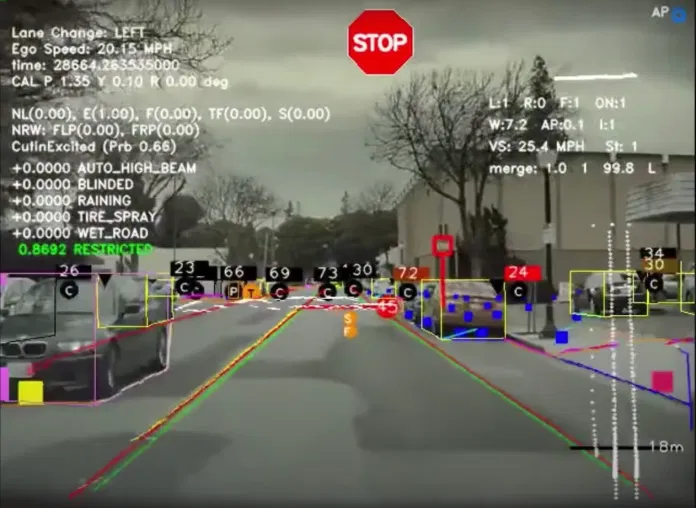
\includegraphics[width=0.9\textwidth]{pictures/Tesla-object-detection.png}
            \caption{Tesla Autopilot object Detection}
            \label{fig:tesla_object_detection}
        \end{figure}
    
        \begin{textblock*}{6cm}(0.88cm,7.4cm)
             \tiny{Source: bdtechtalks, "Tesla AI chief explains why self-driving cars don’t need Lidar"}
        \end{textblock*}
 
        \column{.5\textwidth}
        \begin{figure}
            \centering
            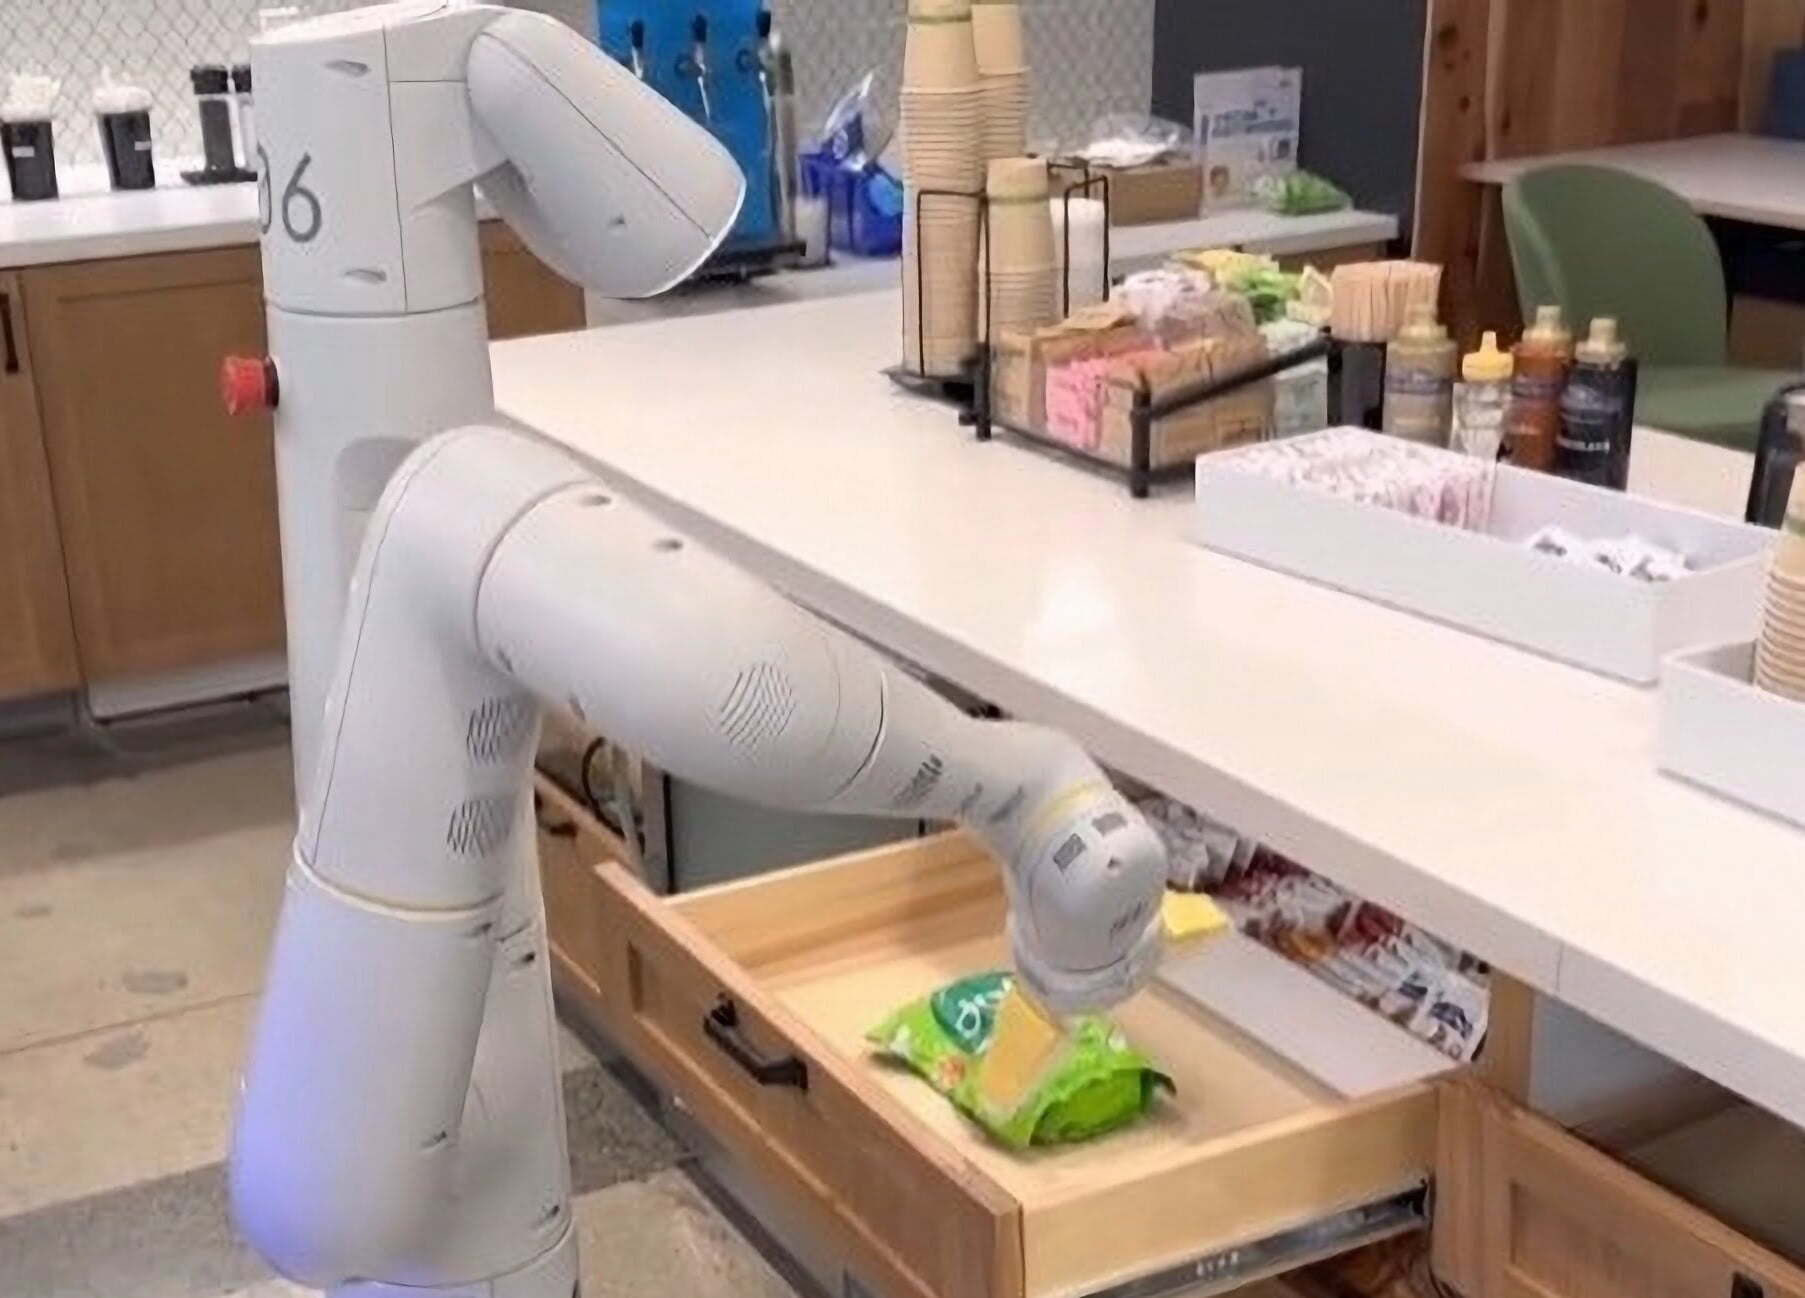
\includegraphics[width=0.9\textwidth]{pictures/palm_e_robot-e1678194832951.jpg}
            \caption{Google PaLm-E robot}
            \label{fig:palm_e_robot}
        \end{figure}

        \begin{textblock*}{6cm}(9.2cm,7.4cm) 
             \tiny{Source: Google Blog "PaLM-E"}
        \end{textblock*}
    \end{columns}
\end{frame}

\begin{frame}{How Computer see}
    \begin{figure}
        \centering
        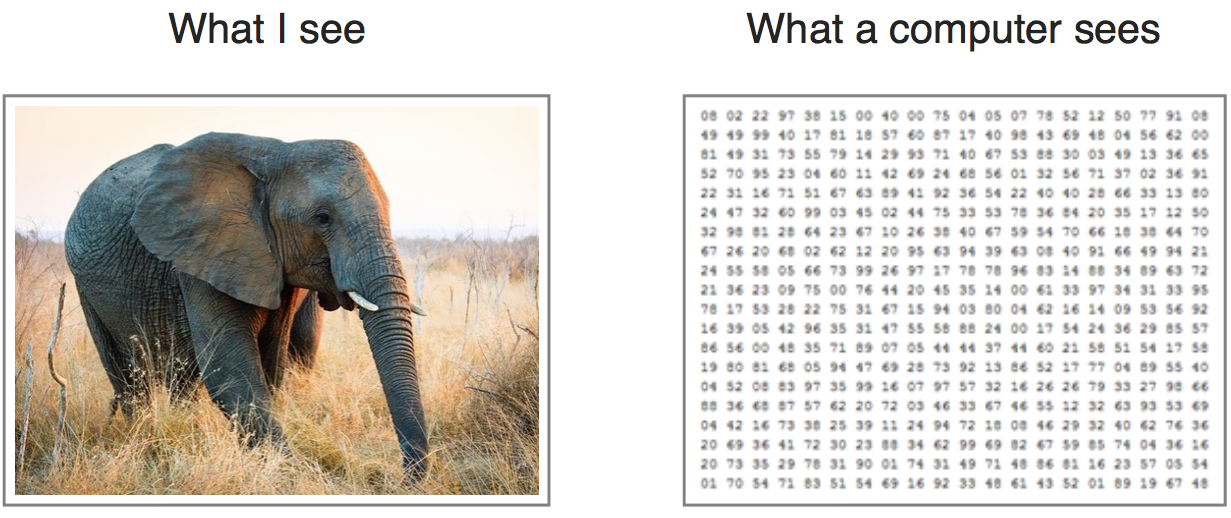
\includegraphics[width=0.9\textwidth]{pictures/what_computer_sees.png}
        \label{fig:what_computer_sees}
    \end{figure} 
        \begin{textblock*}{6cm}(7cm, 8cm) % {block width} (coords) 
             \tiny{Source: GitHub, hosamelsafty/Cats-VS-Dogs}
        \end{textblock*}
\end{frame}

\begin{frame}{Challenges: Viewpoint}
    \begin{columns}
        \column{.7\textwidth}
        \begin{figure}
            \centering
            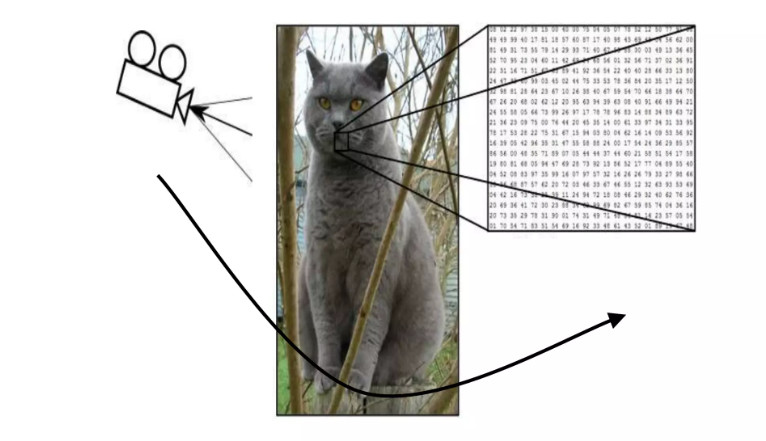
\includegraphics[width=0.9\textwidth]{pictures/viewpoint_variation.png}
            \label{fig:viewpoint_variation}
        \end{figure}
        \begin{textblock*}{6cm}(4.1cm, 7.7cm) % {block width} (coords) 
             \tiny{Source: cs231n, lecture slides}
        \end{textblock*}
        
        \column{0.4\textwidth}
        When we change the viewpoint, \\ all the pixel change!
    \end{columns}
\end{frame}

\begin{frame}{More challenges}
    \begin{itemize}
        \item Viewpoint
        \item Illumination
        \item Occlusions
        \item Background Clutter
        \item etc.
    \end{itemize}
\end{frame}

\begin{frame}{Image Classifier}
    \begin{cyanblock}{}
    \begin{algorithmic}
        \Function{classifyImage}{$Image: Image$}
            \State // What to do here? Magic?
            \State return label
        \EndFunction
    \end{algorithmic}
    \end{cyanblock}

    \vspace{0.3cm}
    It's not obvious how to hard code this.

    \pause
    
    \vspace{0.3cm}
    \textbf{Idea:} Learn how to classify the Images $\longrightarrow$ Use Convolutional Neural Networks(CNN)
\end{frame}

\section{Convolutional Neural Networks(CNN)}

\begin{frame}{CNN Overview}
    \begin{columns}
        \column{0.3\textwidth}
        \begin{itemize}
            \item Used mostly to classify images
            \item A CNN is a specialized NN
            \item It can pick up patterns and make sense 
            \item Consists of the following Components:
            \begin{itemize}
                \item Convolutional Layer 
                \item Pooling Layer
            \end{itemize}
            \item Convolutional Layer consists out of multiple Filters
        \end{itemize}

        \column{0.7\textwidth}
        \begin{figure}
            \centering
            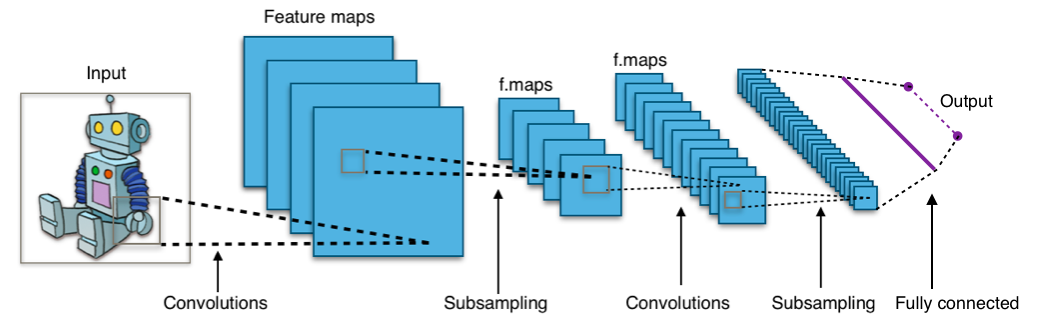
\includegraphics[width=1\textwidth]{pictures/typical_cnn.png}
            \caption{A Typical CNN}
            \label{fig:typical-CNN}
        \end{figure}
         \begin{textblock*}{6cm}(6cm,6.3cm) % {block width} (coords) 
             \tiny{Source: Aphex34, Wikipedia CNN}
        \end{textblock*}

        
    \end{columns}
\end{frame}

\begin{frame}{Patterns}
\begin{columns}
    \column{0.4\textwidth}
    \begin{itemize}
       \item Simple patterns: edges, shapes, textures
       \item More complex patterns: ears, eyes, noses
       \item Even more complex patterns: faces, humans
    \end{itemize}
    These patterns are detected by filters of the Convolutional Layers.
    \column{0.6\textwidth}
    \begin{figure}
        \centering
        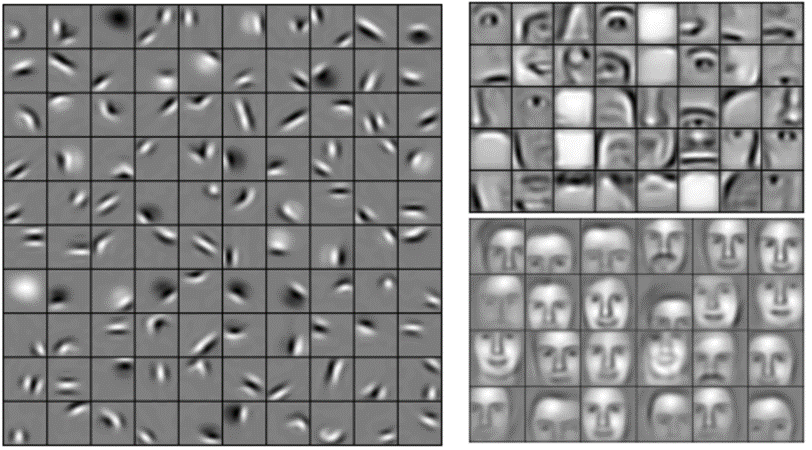
\includegraphics[width=1\textwidth]{pictures/cnn18.png}
        \label{fig:enter-label}
    \end{figure}
    \begin{textblock*}{6cm}(10.5cm, 7.8cm) % {block width} (coords) 
        \tiny{Source: Brandon Rohrer, course 193}
    \end{textblock*}
\end{columns}
\end{frame}

\begin{frame}{Filters/Kernel}
    \begin{columns}
        \column{0.3\textwidth}
        Filter/Kernel: A matrix
        \begin{itemize}
            \item initalized with random values
            \item values adjusted over time, to detect pattern
        \end{itemize}
        Kernel of Convolutional Layer slides over Input
        \column{0.65\textwidth}
        \begin{figure}
            \centering
            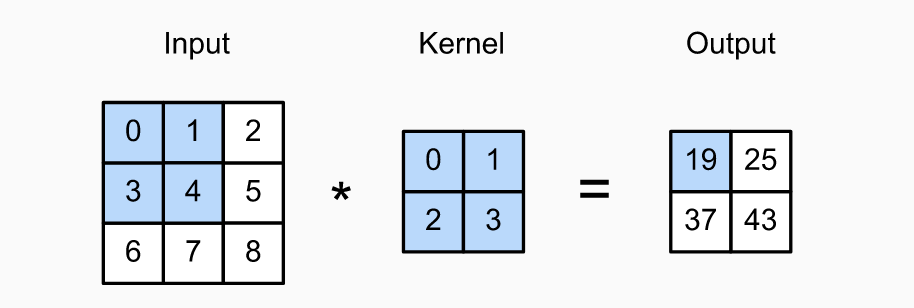
\includegraphics[width=1\textwidth]{pictures/convolution.png}
            \caption{Convolution Operation}
            \label{fig:typical-CNN}
        \end{figure}
         \begin{textblock*}{6cm}(6.2cm,6.6cm) % {block width} (coords) 
             \tiny{Source: d2l.ai, Chapter 7.2}
        \end{textblock*}
    \end{columns}
\end{frame}

\begin{frame}{Convolution}
\begin{columns}
    \column{0.3\textwidth}
    Two Important Hyperparameters:
    \begin{itemize}
        \item Stride
        \item Filter-Size
    \end{itemize}

    \column{0.6\textwidth}
    \begin{figure}
        \centering
        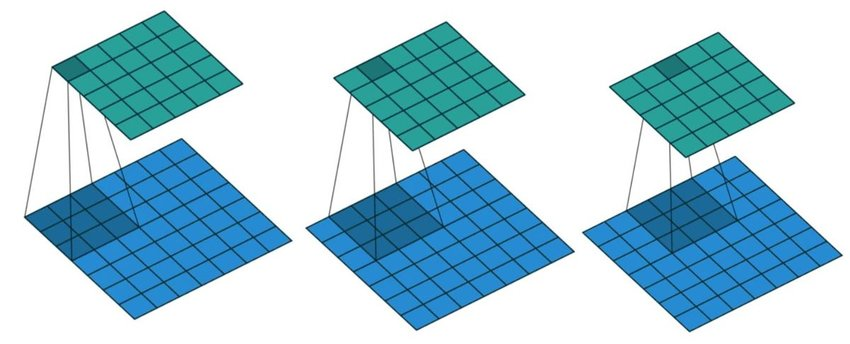
\includegraphics[width=1\textwidth]{pictures/stride1.jpg}
        \caption{A Convolution with Stride 1}
        \label{fig:stride1-conv}
    \end{figure}
    \begin{textblock*}{6cm}(7cm,6.5cm) % {block width} (coords) 
             \tiny{Source: Jelo Salomon, Lung Cancer Detection using Deep Learning}
        \end{textblock*}
\end{columns}
\end{frame}


\begin{frame}{Convolution Animation}
Convolution Animation \\
\\
\tiny{Source: https://youtu.be/xjqCTp4xAtA}
\end{frame}

\begin{frame}{Pooling Layer}
    \begin{itemize}
        \item A way to reduce the dimensionality of our Network
        \begin{itemize}
            \item Requires less computation
        \end{itemize}
        \item Many different ways to do this
        \begin{itemize}
            \item Max-Pooling
            \item Average-Pooling
            \item 1x1 Convolutions
        \end{itemize}
    \end{itemize}
\end{frame}

\begin{frame}{Pooling Layer}
    \begin{figure}
        \centering
        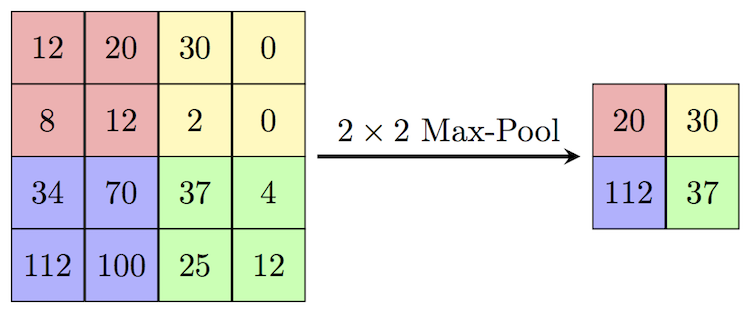
\includegraphics[width=0.7\textwidth]{pictures/Maxpool_sample.png}
        \label{fig:conv_layer}
        \caption{A Max Pooling Layer}
    \end{figure}
    \begin{textblock*}{6cm}(3.2cm, 6.8cm) % {block width} (coords) 
             \tiny{Source: cs231n lecture slides}
    \end{textblock*}
\end{frame}

\begin{frame}{CNN: Bringing it Together}
    \begin{figure}
        \centering
        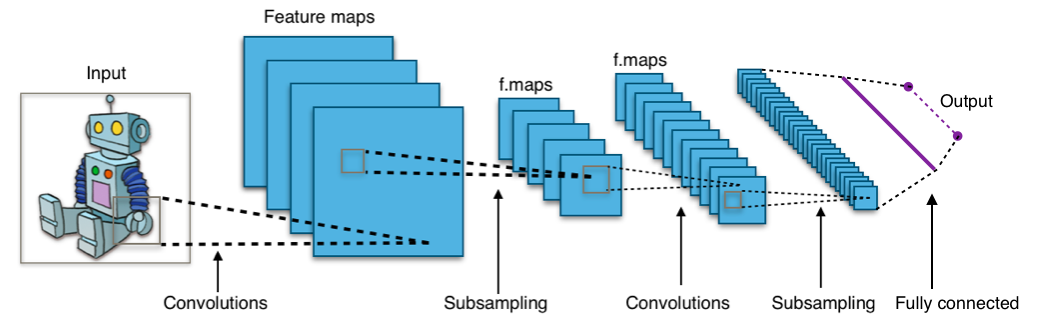
\includegraphics[width=1\textwidth]{pictures/typical_cnn.png}
        \caption{A Typical CNN}
        \label{fig:typical-CNN}
    \end{figure}
\end{frame}


\section{Self-trained CNN}

\begin{frame}{Architecture}
    \begin{figure}
        \centering
        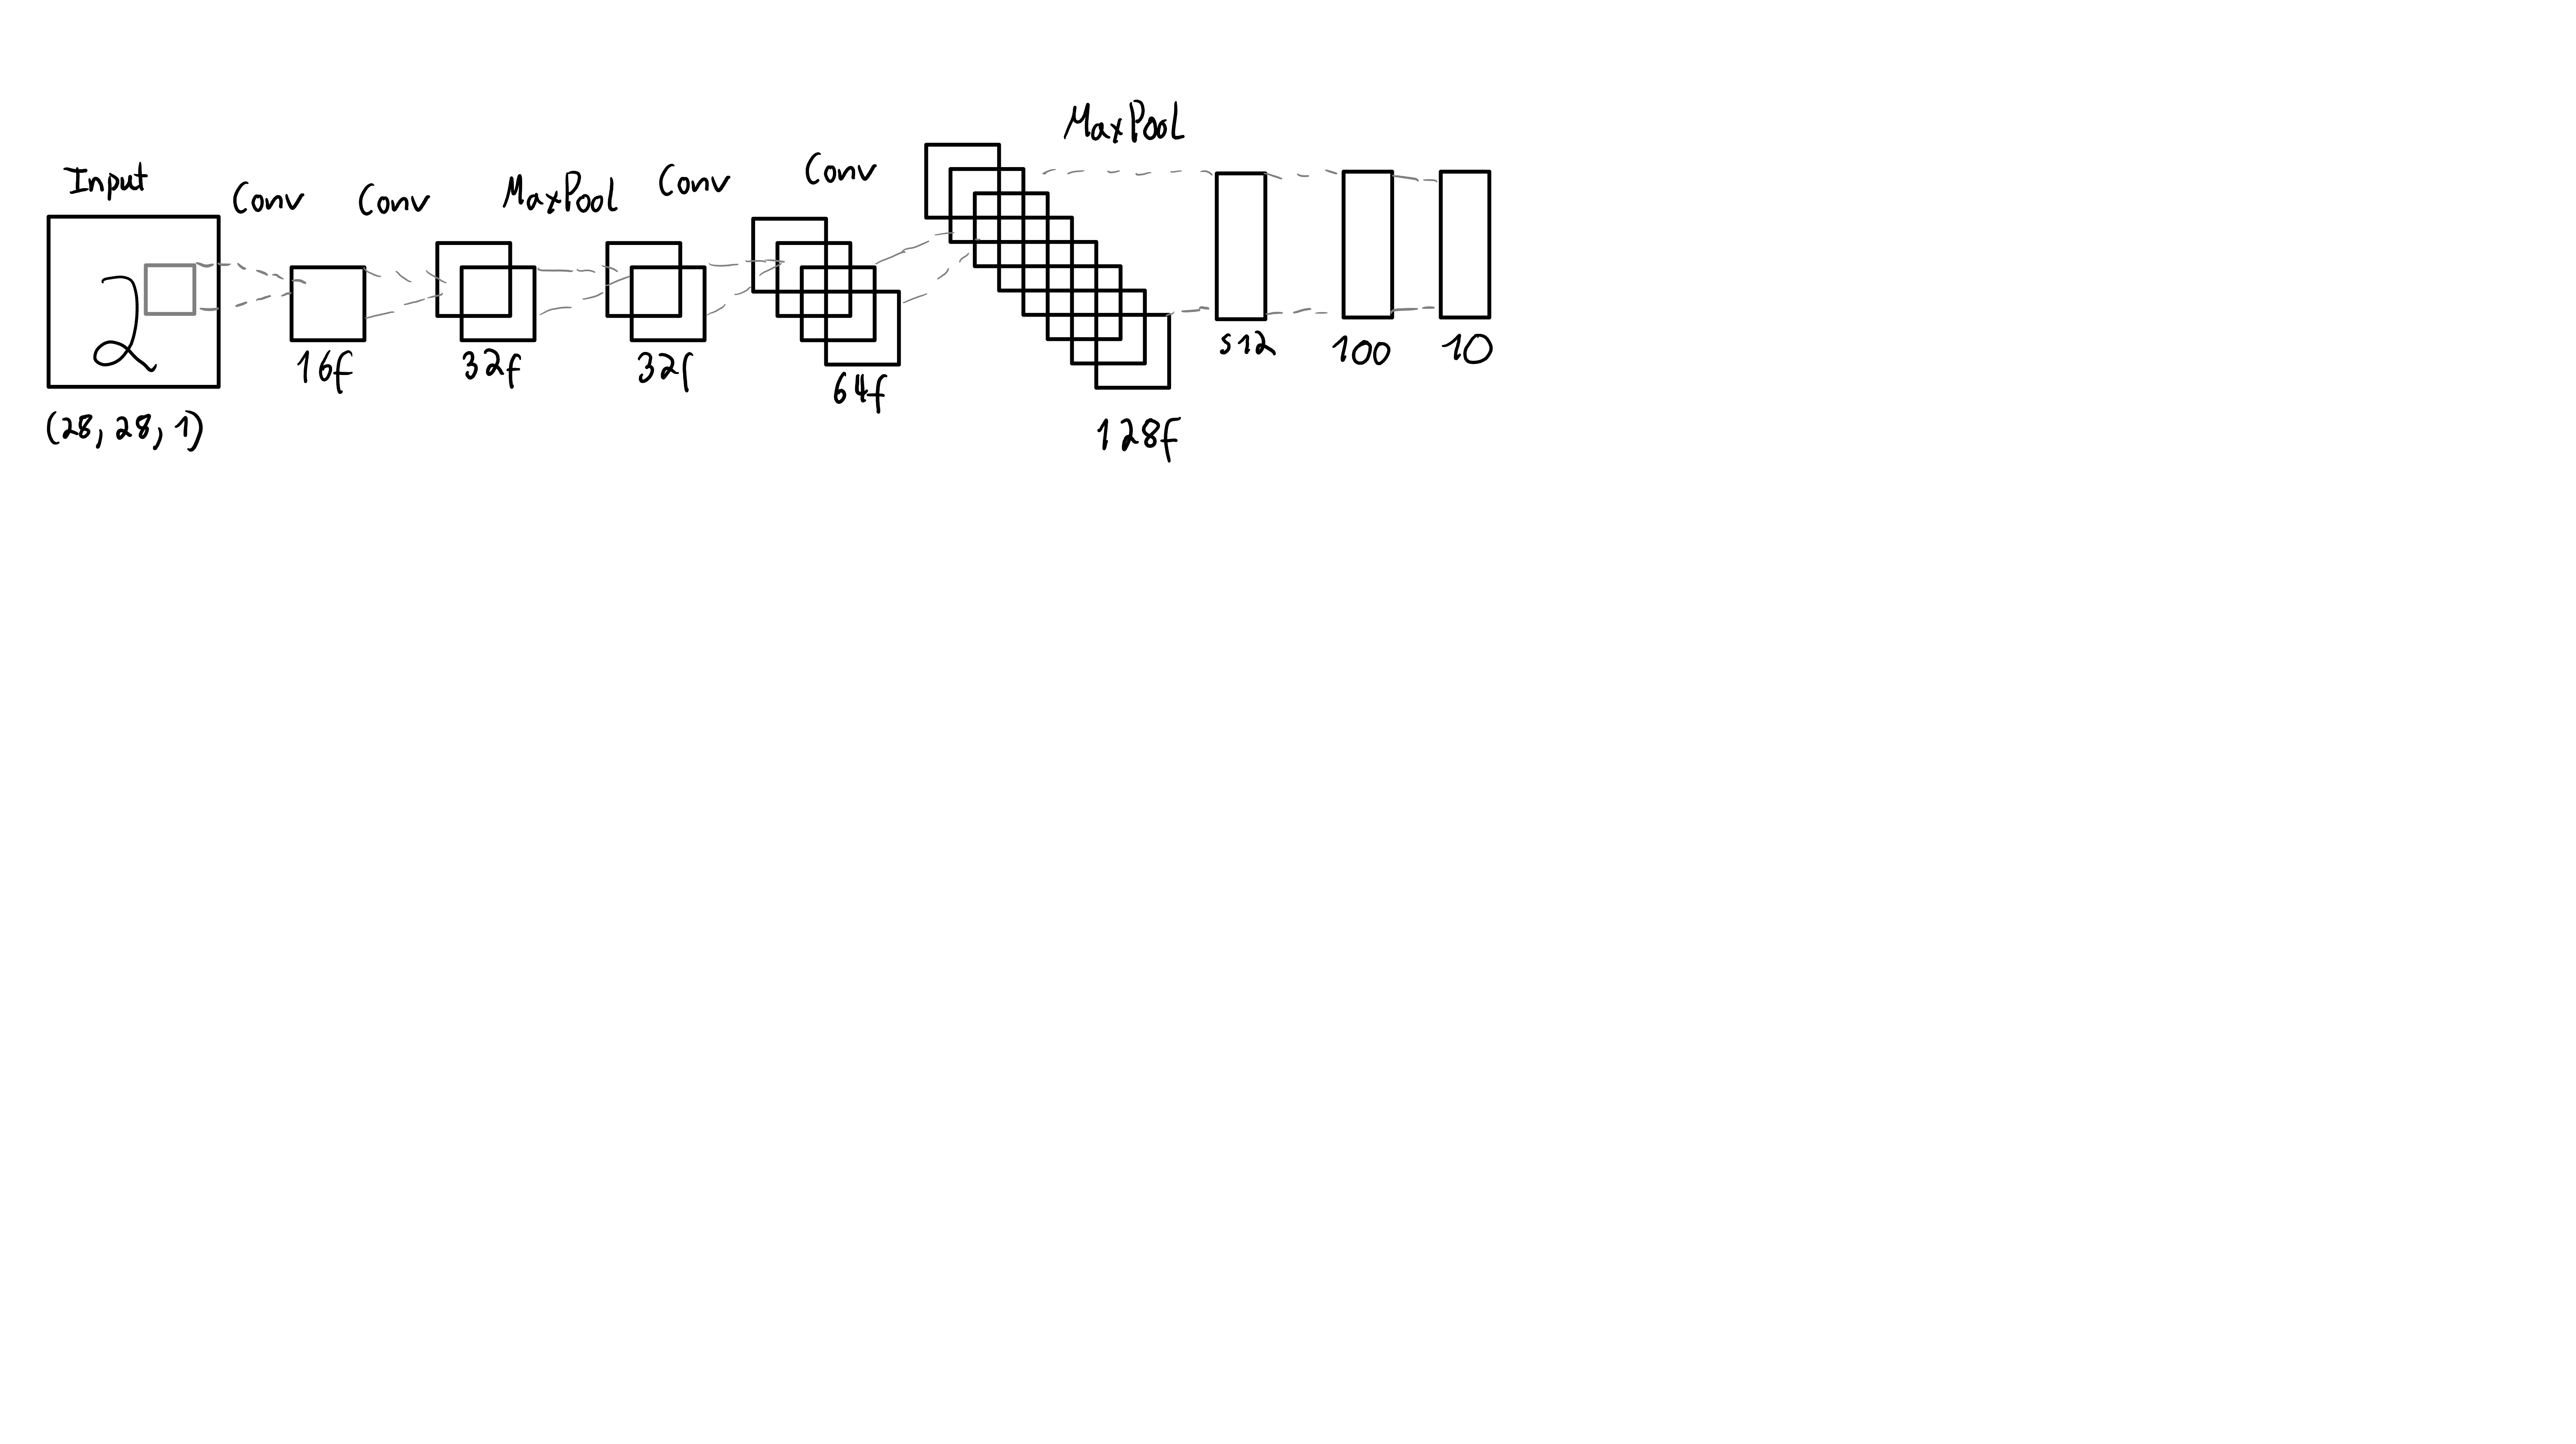
\includegraphics[width=1.75\textwidth]{pictures/architecture_self_trained_new.png}
        \label{fig:self_trained_conv}
    \end{figure}
\end{frame}

\begin{frame}{Trainings-Details}
    \begin{columns}
        \column{.4\textwidth}
        \begin{itemize}
            \item Dataset: MNIST(60,000 Images)
            \item Trainings time: 5 Epochs
            \item Batch size: 1024
            \item Optimizer: Adam
            \item Learning-rate: 0.001
            \item Trained on Google Colab with GPU
        \end{itemize}

        \column{.55\textwidth}
        \begin{figure}
            \centering
            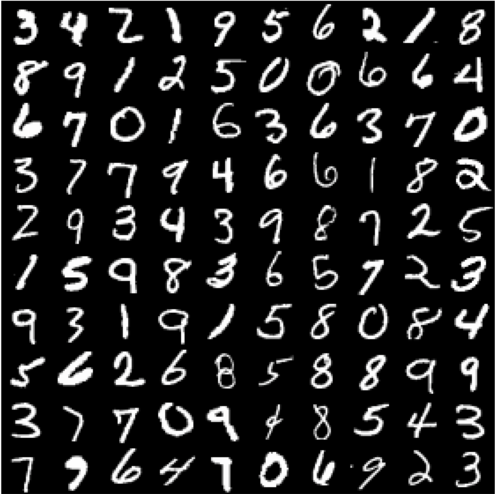
\includegraphics[width=0.6\textwidth]{pictures/mnist.png}
            \label{fig:mnist}
            \caption{Example Data from MNIST dataset}
        \end{figure}
    \end{columns}
\end{frame}

\begin{frame}{Results \& Ablation}
    \vspace{-40pt}
    \begin{figure}
        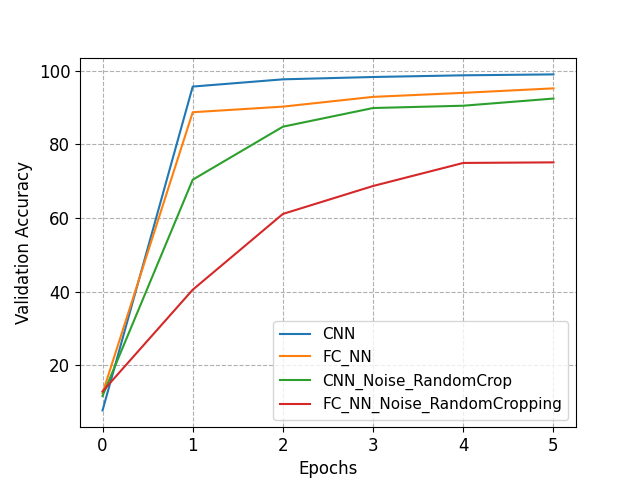
\includegraphics[width=0.65\textwidth]{pictures/val_acc_result_data.png}
    \end{figure}
\end{frame}

\section{Summary}
\begin{frame}{Summary}
\begin{itemize}
    \item Teaching a Computer the semantic meaning of Images is hard
    \pause
    \item But it's possible with the help of CNN
    \pause
    \item Nowdays its rather easy to get good performance on simple datasets
\end{itemize}
\end{frame}

\appendix
\beginbackup

\begin{frame}{Literature}
\nocite{*} % prints all papers in bib, even if not cited
\printbibliography
\end{frame}
\end{document}
